\documentclass{scrartcl}

\usepackage{ucs}
\usepackage[utf8x]{inputenc}
\usepackage[ngerman]{babel}
\usepackage{graphicx}
\usepackage{amsmath}
\usepackage{amssymb}
\usepackage{color}
\usepackage[table]{xcolor}
\definecolor{lightgray}{rgb}{.9,.9,.9}
\definecolor{darkgray}{rgb}{.4,.4,.4}
\usepackage{listings}
\usepackage{multicol}
\usepackage[export]{adjustbox}
\usepackage{longtable}

\lstdefinelanguage{PVS}{
	keywords={ theory, begin, recursive, if, then, else, endif, measure, theorem, forall, end, type, cases, of, endcases, exists, type+, importing, lemma, axiom, var, assuming, lambda, true, false, and, or, implies, iff, not, by, nonempty\_type, from },
	keywordstyle=\color{blue}\bfseries,
	sensitive=false,
	comment=[l]{\%},
	commentstyle=\color{darkgray}\ttfamily,
	stringstyle=\color{red}\ttfamily,
	morestring=[b]"
}

\lstset{
	language=PVS,
	backgroundcolor=\color{lightgray},
	extendedchars=true,
	basicstyle=\footnotesize\ttfamily,
	showstringspaces=false,
	showspaces=false,
	numbers=left,
	numberstyle=\footnotesize,
	numbersep=9pt,
	tabsize=2,
	breaklines=true,
	showtabs=false,
	captionpos=b
}

\lstset{literate=%
	{Ö}{{\"O}}1
	{Ä}{{\"A}}1
	{Ü}{{\"U}}1
	{ß}{{\ss}}1
	{ü}{{\"u}}1
	{ä}{{\"a}}1
	{ö}{{\"o}}1
	{~}{{\textasciitilde}}1
}

\setlength\parindent{0pt}

\newcommand*\xor{\mathbin{\oplus}}

\title{Rechnergestützte Beweissysteme \\ Zusammenfassung}
\author{Thomas Mohr}
\date{}

\begin{document}
\maketitle

\section{PVS - Prototype Verification System}

\begin{lstlisting}
	sum : THEORY BEGIN
	
		% Rekursive Definition der Summe aller Zahlen von 0 bis n
		sum_fun(n : nat) : RECURSIVE nat =
			IF n = 0 THEN 0
			ELSE summe(n - 1) + n
			ENDIF
			MEASURE n
			
		gauss : THEOREM
			FORALL(n : nat):
				2 * summe(n) = n * (n + 1)
				
	END sum
\end{lstlisting}

\begin{lstlisting}
	dfa [
		Zeichen		: TYPE,
		Zustand		: TYPE,
		
		start			: Zustand,
		delta			: [Zustand,Zeichen->Zustand],
		terminal	: set[Zustand]
	] : THEORY BEGIN
	
		Wort : TYPE = list[Zeichen]
		
		deltaStar(z : Zustand, w : Wort) : RECURSIVE Zustand =
			CASES w OF
				null		: z,
				cons(a,v)	: delta(deltaStar(z,v), a)
			ENDCASES
			MEASURE length(w)
			
		dAccept(w : Wort) : bool =
			terminal(deltaStar(start,w))
	
	END dfa
\end{lstlisting}

\subsection{Sequenzen}

\begin{equation*}
	H_1, H_2, \ldots, H_n \vdash G_1, G_2, \ldots, G_k
\end{equation*}

Dabei sind $ H_1, \ldots, H_n \vdash G_1, \ldots, G_k $ logische Formeln. \\
Die Folge $ H_1, \ldots, H_n $ heißt ''Antezedent'', die Folge $ G_1, \ldots, G_k $ ''Sukkzedent''. \\

Die Beweisaufgabe besteht darin, aus der \textbf{Konjunktion} der Hypothesen $ H_1, \ldots, H_n $ die \textbf{Disjunktion} der Zielformeln (\textit{goal formulae})  $ G_1, \ldots, G_k $ zu beweisen. \\

Die \textbf{Semantik} (Bedeutung) der obigen Sequenz ist also:

\begin{equation*}
	H_1 \wedge H_2 \wedge \ldots \wedge H_n \implies G_1 \vee G_2 \vee \ldots \vee G_k
\end{equation*}

Sequenzen werden in PVS folgendermaßen dargestellt

\begin{align*}
	[-1] H_1 \\
	\ldots \\
	[-n] H_n \\
	|------- \\
	[1] G_1 \\
	\ldots \\
	[k] G_k
\end{align*}

Durch die vorangestellten Nummern $ -1,\ldots,-n,1,\ldots,k $ können sich Beweisbefehle auf einzelne Formeln der Sequenz beziehen. Mit ''+'' bezieht man sich auf alle Formeln im Sukkzedent, mit ''-'' auf alle Formeln im Antezedenz. \\

\renewcommand{\arraystretch}{2}
\begin{tabular}{l|l}
	\textbf{(split k)} & Wende \textbf{split} auf k-te Zielformel an \\
	\hline
	\textbf{(split -k)} & Wende \textbf{split} auf k-te Hypothese an \\
	\hline
	\textbf{(split +)} & Wende \textbf{split} auf alle Formeln im Sukkzedenz an \\
	\hline
	\textbf{(split -)} & Wende \textbf{split} alle Formeln im Antezenenz an \\
	\hline
	\textbf{(split)} & Wende \textbf{split} überall an \\
	\hline
	\textbf{(split (k1 k2 $ \ldots $ kn))} & Wende \textbf{split} auf die angegebenen Formeln an
\end{tabular}

\subsection{Beweisbefehle}

\renewcommand{\arraystretch}{2}
\begin{tabular}{l|l}
	\textbf{(flatten)} & Entspricht den $ \alpha $-Regeln im Tableaukalkül \\
	\hline
	\textbf{(split)} & Entspricht den $ \beta $-Regeln im Tableaukalkül \\
	\hline
	\textbf{(prop)} & Kombiniert \textbf{(flatten)} und \textbf{(split)} mehrfach \\
	\hline
	\textbf{(case $ p $)} & Fallunterscheidung. $ p \vee \neg p $ in die Hypothesen aufnehmen \\
	\hline
	\textbf{(lemma hilfssatz)} & Nutzt das Lemma (Axiom, etc.) ''hilfssatz'' als Antezedent \\
	\hline
	\textbf{(expand func)} & Expandiert die Funktion ''func'' \\
	\hline
	\textbf{(copy $ x $)} & Kopiert Zeile $ x $ \\
	\hline
	\textbf{(hide $ x $)} & Entfernt Zeile $ x $ \\
	\hline
	\textbf{(postpone)} & Stellt eine Beweisaufgabe temporär zurück \\
	\hline
	\textbf{(skolem)} & Skolemisieren ($ \forall $-right, $ \exists $-left) \\
	\hline
	\textbf{(skeep)} & Wie \textbf{(skolem)}, nur bleiben Variablennamen gleich \\
	\hline
	\textbf{(inst ''$ x $'')} & Instanziiert Terme ($ \forall $-left, $ \exists $-right) mit $ x $ \\
	\hline
	\textbf{(inst-cp ''$ x $'')} & Wie \textbf{(inst)}, nur kopiert es den Term vor der Instanziierung \\
	\hline
	\textbf{(lift-if)} & f(if $ b $ then $ t_1 $ else $ t_2 $) $ \rightarrow $ if $ b $ then f($ t_1 $) else f($ t_2 $), falls $ t_1,t_2:\tau $ \\
	\hline
	\textbf{(replace source target)} & Substitution (Standard: Links nach Rechts) \\
	\hline
	\textbf{(replace source target :dir rl)} & Wie \textbf{(replace)}, nur von Rechts nach Links \\
	\hline
	\textbf{(extensionality $ \tau $)} & Führt ein Extensionalitätslemma für $ \tau $ in den Beweis ein \\
	\hline
	\textbf{(induct $ n $)} & Induktion über $ n $ \\
	\hline
	\textbf{(induct-and-simplify n)} & Induktion über $ n $ mit anschließenden Vereinfachungen \\
	\hline
	\textbf{(typepred ''$ x $'')} & Führt die Subtypeneinschränkung für $ x $ als Antezedenz ein
\end{tabular}

\pagebreak
\subsection{=-Relation}

\begin{itemize}
	\item Die Relation ''='' kommt in den meisten praktischen Spezifikationen vor
	\item Um sie nicht mit dem metasprachlichen ''='' zu verwechseln, nennen wir sie ''$ \triangleq $''
	\item Statt $ \triangleq(t_1,t_2) $ schreibt man $ t_1 \triangleq t_2 $ (Infix statt Präfix)
	\item Axiome $ Ax_\triangleq $
	\begin{itemize}
		\item Äquivalenzrelation \\
		\renewcommand{\arraystretch}{2}
		\begin{tabular}{l|l}
			$ \forall x.x \triangleq x $ & Reflexivität \\ 
			\hline 
			$ \forall x,y.x \triangleq y \implies y \triangleq x $ & Symmetrie \\ 
			\hline 
			$ \forall x,y,z.x \triangleq y \wedge y \triangleq z \implies x \triangleq z $ & Transitivität
		\end{tabular} 
		\item Kongruenzrelation, d.h. für jedes $ f \in \mathcal{F} $ und für jedes $ R \in \mathcal{R} $ gilt:
		\begin{enumerate}\addtocounter{enumi}{3}
			\item $ \forall x_1,\ldots,x_n \forall y_1,\ldots,y_n.x_1 \triangleq y_1 \wedge \ldots \wedge x_n \triangleq y_n $ \\
			$ \implies f(x_1,\ldots,x_n) \triangleq f(y_1,\ldots,y_n) $
			\item $ \forall x_1,\ldots,x_n \forall y_1,\ldots,y_n.x_1 \triangleq y_1 \wedge \ldots \wedge x_n \triangleq y_n $ \\
			$ \implies R(x_1,\ldots,x_n) \triangleq R(y_1,\ldots,y_n) $
		\end{enumerate}
	\end{itemize}
\end{itemize}

\subsection{Substitutionslemma für Terme}

\begin{itemize}
	\item Unter der Voraussetzung der Gleichheitsaxiome gilt für beliebige Terme $ t $
	\begin{itemize}
		\item $ t_1 \triangleq t_2 \implies t\{ t_1/x \} \triangleq t\{ t_2/x \} $
		\item $ t_1 \triangleq t_2 \implies (F\{ t_1/x \} \iff F\{ t_2/x \}) $
	\end{itemize}
\end{itemize}

\pagebreak
\section{Aussagenlogische Berechnungen}

\subsection{Tseitin Transformation}

Die Umwandlung einer Formel $ F $ in eine Menge von Klauseln, z.B. durch Umführung in Normalform (KNF/DNF), kann sehr ineffizient sein und führt im schlimmsten Fall zu $ 2^n $ Klauseln. Alternativ kann die Tseitin Transformation verwendet werden, bei der jede Klausel höchstens 3 Literale enthält. Nachteil der Tseitin Transformation ist jedoch, dass durch eine Vielzahl an Umbenennungen zusätzliche Variablen erstellt werden. \\

\begin{itemize}
	\item Zu einer aussagenlogischen Formel $ F $ wird eine Klauselmenge $ \mathcal{K} $ gefunden, so dass gilt
	\begin{itemize}
		\item $ F $ ist erfüllbar $ \iff \mathcal{K} $ ist erfüllbar
		\item Jede Klausel $ k \in \mathcal{K} $ hat höchstens 3 Literale
	\end{itemize}
	\item Vorsicht
	\begin{itemize}
		\item Keine Äquivalenzumwandlung
		\item $ F \not \equiv \wedge_{k \in \mathcal{K}} k $
		\item Insbesondere hat $ \mathcal{K} $ i.A. mehr Variablen als $ F $
	\end{itemize}
	\item Idee
	\begin{itemize}
		\item Ersetze alle Operatoren $ l_1 \odot l_2 $ in $ F $, wobei $ l_1 $ und $ l_2 $ Literale sind, durch eine neue Variable $ v $ und erzeuge eine Klauselmenge, die äquivalent ist zu $ v \iff l_1 \odot l_2 $.
		\item Wiederhole dies, bis $ F $ keinen Operator mehr enthält
	\end{itemize}
\end{itemize}

\begin{align*}
	F = (b \vee a \wedge c) \xor ((a \vee b) \wedge (b \vee c))
\end{align*}

\begin{itemize}
	\item Ersetze Operatoren durch Gleichungen
	\begin{enumerate}
		\item $ (x \iff a \wedge c) $
		\item $ (y \iff b \vee x) $
		\item $ (u \iff a \vee b) $
		\item $ (v \iff b \vee c) $
		\item $ (w \iff u \wedge v) $
		\item $ o \iff y \xor w $
	\end{enumerate}
	\item Ersetze jede Gleichung durch äquivalente Klauselmenge
	\begin{equation}
		\begin{split}
			(x \iff a \wedge c) &= (x \implies a \wedge c) \wedge (a \wedge c \implies x) \\
			&= (\neg x \vee a \wedge c) \wedge (\neg (a \wedge c) \vee x) \\
			&= (\neg x \vee a \wedge c) \wedge ((\neg a \vee \neg c) \vee x) \\
			&= (\neg x \vee a \wedge c) \wedge (\neg a \vee \neg c \vee x) \\
			&= (\neg x \vee a) \wedge c \wedge (\neg a \vee \neg c \vee x) \\
			&\equiv \{ \{ \overline{x},a \},\{ c \},\{ \overline{a},\overline{c},x \} \}
		\end{split}
	\end{equation}
	\begin{equation}
		\begin{split}
			(y \iff b \vee x) &= (x \implies b \vee x) \wedge (b \vee x \implies y) \\
			&= (\neg x \vee (b \vee x)) \wedge (\neg (b \vee x) \vee y)) \\
			&= (\neg x \vee b \vee x) \wedge ((\neg b \wedge \neg x) \vee y) \\
			&= (\neg x  \vee b \vee x) \wedge (\neg b \vee y) \wedge (\neg x \vee y) \\
			&\equiv \{ \{ \overline{x},b,c \},\{ \overline{b},y \},\{ \overline{x},y \} \}
		\end{split}
	\end{equation}
	\begin{equation}
		\begin{split}
			(u \iff a \vee b) &= (u \implies a \vee b) \wedge (a \vee b \implies u) \\
			&= (\neg u \vee a \vee b) \wedge (\neg (a \vee b) \vee u) \\
			&= (\neg u \vee a \vee b) \wedge ((\neg a \wedge \neg b) \vee u) \\
			&= (\neg u \vee a \vee b) \wedge (\neg a \vee u) \wedge (\neg b \vee u) \\
			&\equiv \{ \{ \overline{u},a,b \},\{ \overline{a},u \},\{ \overline{b},u \} \}
		\end{split}
	\end{equation}
	\begin{equation}
		\begin{split}
			(v \iff b \vee b) &= (u \implies b \vee c) \wedge (b \vee c \implies v) \\
			&= (\neg v \vee b \vee c) \wedge (\neg (b \vee c) \vee v) \\
			&= (\neg v \vee b \vee c) \wedge ((\neg b \wedge \neg c) \vee v) \\
			&= (\neg v \vee b \vee c) \wedge (\neg b \vee v) \wedge (\neg c \vee v) \\
			&\equiv \{ \{ \overline{v},b,c \},\{ \overline{b},v \},\{ \overline{c},v \} \}
		\end{split}
	\end{equation}
	\begin{equation}
		\begin{split}
			(w \iff u \wedge v) &= (x \implies a \wedge v) \wedge (u \wedge v \implies w) \\
			&= (\neg w \vee u \wedge v) \wedge (\neg (u \wedge v) \vee w) \\
			&= (\neg w \vee u \wedge v) \wedge ((\neg u \vee \neg v) \vee w) \\
			&= (\neg w \vee u \wedge v) \wedge (\neg u \vee \neg v \vee w) \\
			&= (\neg w \vee u) \wedge v \wedge (\neg u \vee \neg v \vee w) \\
			&\equiv \{ \{ \overline{w},u \},\{ v \},\{ \overline{u},\overline{v},w \} \}
		\end{split}
	\end{equation}
	\begin{equation}
		\begin{split}
			o \iff y \xor w &= (y \vee w) \wedge \neg (y \wedge w) \\
			&= (y \vee w) \wedge (\neg y \vee \neg w) \\
			&\equiv \{ \{ y,w \},\{ \overline{y},\overline{w} \} \}
		\end{split}
	\end{equation}
\end{itemize}

Da in der finalen Klauselmenge $ \mathcal{K}(o) $ (KNF) sowohl $ \{ y,w \} $, als auch $ \{ \overline{y},\overline{w} \} $ enthalten sind ist die Klauselmenge unerfüllbar und damit auch die ursprüngliche Formel unerfüllbar.

\pagebreak
\subsection{Shannon-Expansion}

\begin{align*}
	\textcolor{red}{if}(A) \, \textcolor{red}{then} \, B \, \textcolor{red}{else} \, C := (A \wedge B) \vee (\neg A \wedge C)
\end{align*}

\underline{Lemma}: Für jede Formel $ F $ und jedes Atom $ A_i $ gilt: $ F \equiv if \, (A_i) \, then \, F_{[\top / A_i]} \, else \, F_{[\bot / A_i]} $ \\

\underline{Beweis}: Für jede passende Belegung $ \alpha $ gilt:

\begin{enumerate}
	\item Falls $ \alpha(A_i) = 1 $:
	\begin{align*}
		\alpha(A_i) \wedge \alpha(F_{[\top / A_i]}) \vee \neg \alpha(A_i) \wedge \alpha(F_{[\bot / A_i]}) &= \alpha(F_{[\top / A_i]}) \\
		&= \alpha_{[A_i \mapsto 1]}(F) \\
		&= \alpha(F)
	\end{align*}
	\item Falls $ \alpha(A_i) = 0 $: analog.
\end{enumerate}

\section{Typen und Typinferenz}

\subsection{Kontexte}

\begin{itemize}
	\item Kontext: Abbildung von Variablen in Typen:
	\begin{equation*}
		K = \{ x_1 : \tau_1, \ldots, x_n : \tau_n \}
	\end{equation*}
	bedeutet:
	\begin{equation*}
		K(x_1) = \tau_1, \ldots, K(x_n) = \tau_n
	\end{equation*}
	\item Wir schreiben $ K \triangleright t : \tau $ falls im Kontext $ K $ der Term $ t $ den Typ $ \tau $ hat.
	\item Die folgenden Schlussregeln definieren die Syntax von Termen und gleichzeitig deren Typ im Kontext $ K $: \\
	
	\begin{minipage}{.5\linewidth}
		\begin{equation*}
		\frac{K(x) = t}{K \triangleright x : t}
		\end{equation*}
	\end{minipage}
	\begin{minipage}{.5\linewidth}
		''Jede Variable vom Typ $ \tau $ ist auch ein Term vom Typ $ \tau $''
	\end{minipage}
	
	\begin{minipage}{.5\linewidth}
		\begin{equation*}
			\frac{K \triangleright t_1 : \tau_1, \ldots, K \triangleright t_n : \tau_n}{K \triangleright f(t_1, \ldots, t_n) : \tau}
		\end{equation*}
	\end{minipage}
	\begin{minipage}{.5\linewidth}
		falls $ f : \tau_1 \times \ldots \times \tau_n \rightarrow \tau $
	\end{minipage}
\end{itemize}

\subsubsection{IF und ''=''}

\begin{itemize}
	\item Für jeden Typ $ \tau $ hat PVS automatisch die Terme
	\begin{itemize}
		\item IF\_THEN\_ELSE : $ [bool, \tau, \tau \rightarrow \tau] $
		\item = : $ [\tau, \tau \rightarrow bool] $
	\end{itemize}
	\item mit den Typ-Regeln \\
	
	\begin{minipage}{.5\linewidth}
		\begin{equation*}
		\frac{K \triangleright t_1 : bool, K \triangleright t_2 : \tau, K \triangleright t_3 : \tau}{K \triangleright (IF \, t_1 \, THEN \, t_2 \, ELSE \, t_3) : \tau}
		\end{equation*}
	\end{minipage}
	\begin{minipage}{.5\linewidth}
		\begin{equation*}
		\frac{K \triangleright t_1 : \tau, K \triangleright t_2 : \tau}{K \triangleright t_1 = t_2 : bool}
		\end{equation*}
	\end{minipage}
\end{itemize}

\subsubsection{Atomare Ausdrücke}

\begin{itemize}
	\item Atomare Ausdrücke sind die elementaren Ausdrücke der Prädikatenlogik. Ein atomarer Ausdruck $ R(t_1,\ldots,t_n) $ besagt, dass $ t_1,\ldots,t_n $ in der Relation $ R $ stehen. Für jede Relation $ R $ hat man also eine Typregel \\
	
	\begin{minipage}{.5\linewidth}
		\begin{equation*}
			\frac{K \triangleright t_1 : \tau_1,\ldots,K \triangleright t_n : \tau_n}{K \triangleright R(t_1,\ldots,t_n) : bool}
		\end{equation*}
	\end{minipage}
	\begin{minipage}{.5\linewidth}
		,falls $ R :: \tau_1 \times \ldots \times \tau_n $.
	\end{minipage}
\end{itemize}

\subsection{Typen in PVS}

\subsubsection{Eingebaute PVS-Typen}

\begin{tabular}{|c|c|}
	\hline 
	bool & $ \mathbb{B} $ \\ 
	\hline 
	nat & $ \mathbb{N} $ \\ 
	\hline 
	int & $ \mathbb{Z} $ \\ 
	\hline 
	rat & $ \mathbb{Q} $ \\ 
	\hline 
	real & $ \mathbb{R} $ \\ 
	\hline 
\end{tabular} 

\subsubsection{Uninterpretierte PVS-Typen}

\begin{itemize}
	\item Uninterpretierte Typen werden durch das Schlüsselwort \textcolor{blue}{TYPE} eingeführt
	\begin{lstlisting}
H : TYPE % H sei eine beliebige Menge
	\end{lstlisting}
	\item In PVS kann ein Typ auch leer sein
	\item Nichtleere Typen sepzifiziert durch \textcolor{blue}{TYPE+}
	\begin{lstlisting}
G : TYPE+ % G sei eine nichtleere Menge
	\end{lstlisting}
	\item Wenn ein Typ eine Konstante haben soll, muss er nichtleer sein
	\begin{lstlisting}
G		: TYPE+
e		: G
o		: [G,G->G]
inv	: [G->G]
	\end{lstlisting}
\end{itemize}

\subsubsection{Uninterpretierte Teil-Typen}

\begin{itemize}
	\item Uninterpretierte Teil-Typen können zu jedem vorhandenen Typ durch das Schlüsselwort \textcolor{blue}{TYPE FROM} erklärt werden.
	\begin{lstlisting}
H	: TYPE					% H sei eine beliebige Menge
S	: TYPE FROM H		% S ist ein Teiltyp von H
F	: TYPE FROM nat	% F sei eine Teilmenge der natürlichen Zahlen
	\end{lstlisting}
	\item Nichtleere Teil-Typen durch \textcolor{blue}{NONEMPTY\_TYPE FROM}
	\begin{lstlisting}
G	: TYPE+										% G sei eine nichtleere Menge
H	: NONEMPTY_TYPE FROM G		% H sei nichtleere Teilmenge von G
M	: NONEMPTY_TYPE FROM nat	% M sei nichtleere Teilmenge
														% der natürlichen Zahlen
	\end{lstlisting}
\end{itemize}

\subsubsection{Aufzählungstypen}

\begin{itemize}
	\item Aufzählungstypen werden durch Angabe der möglichen Werte definiert
	\begin{lstlisting}
Farbe : TYPE = { rot, grün, blau }
	\end{lstlisting}
	\item \textcolor{blue}{bool} ist ein Aufzählungstyp mit den Werten TRUE, FALSE
\end{itemize}

\subsubsection{Kartesisches Produkt}

\begin{itemize}
	\item $ T_1, T_2, \ldots, T_n $ seien beliebige Typen
	\item Kartesische Produkt (tuple type): \textcolor{blue}{$ [T_1,T_2,\ldots,T_n] $}
	\item Bedeutung: $ T_1 \times T_2 \times \ldots \times T_n $
	\item Konstruktor: \textcolor{blue}{$ (\ldots, \ldots, \ldots) $}
	\item Selektoren: \textcolor{blue}{$ proj_1, \ldots, proj_n $} alternativ \textcolor{blue}{$ '1, \ldots, 'n $}
	\begin{lstlisting}
Rational : TYPE = [nat,nat]	% ein Rational ist ein paar
														% von natürlichen Zahlen
(3,5) : Rational						% (3,5) ist ein Rational
IF x = (3,5) THEN proj_1(x) = 3
(3,5)'2 = 5 
	\end{lstlisting}
\end{itemize}

\subsubsection{Recordtypen}

\begin{itemize}
	\item Recordtypen \textcolor{blue}{$ [\# \, name_1 : T_1, name_2 : T_2, \ldots, name_n : T_n \, \#] $}
	\item Bedeutung: \textcolor{blue}{$ T_1 \times T_2 \times \ldots \times T_n $} mit selbstgewählten Namen für den Zugriff auf die Komponenten
	\item Konstruktor: \textcolor{blue}{$ (\# \, \ldots, \ldots, \ldots \, \#) $}
	\item Selektoren: \textcolor{blue}{$ name_1, \ldots, name_n $} als einstellige Funktionen
	\begin{lstlisting}
Rational	: TYPE = [# zähler : nat, nenner : nat #]
(# zähler := 3, nenner := 5 #) = (# nenner := 5, zähler := 3 #)
IF x = (# zähler := 3, nenner := 5 #) THEN zähler(x) = 3
nenner((# zähler := 3, nenner := 5 #)) = 5
	\end{lstlisting}
\end{itemize}

\subsubsection{Funktionstypen}

\begin{itemize}
	\item Funktionstypen (function type) \textcolor{blue}{$ [T_1 \rightarrow T_2] $}
	\item Bedeutung: \textcolor{blue}{$ [T_1 \rightarrow T_2] $} ist die Menge aller Abbildungen von $ T_1 $ nach $ T_2 $. Abbildungen mit mehreren Argumenten in Verbindung mit Tupeln: \\
	\textcolor{blue}{$ [T_1,T_1 \rightarrow T_2] $} ist Kurzform für \textcolor{blue}{$ [[T_1,T_1] \rightarrow T_2] $}
	\item Konstruktor: \textcolor{blue}{$ (LAMBDA(v : T_1) : t) $}, wobei $ v $ eine Variable und $ t $ ein Term vom Typ $ T_1 $ ist
	\item Selektor: Funktionsapplikation \textcolor{blue}{f(t)}, wobei $ f : [T_1 \rightarrow T_2] $ und $ t $ Term vom Typ $ T_1 $
	\begin{lstlisting}
(LAMBDA(x : nat) : x + 1): [nat->nat]
(LAMBDA(x,y : nat): x*x+y*y) : [nat,nat->nat]
IF f = (LAMBDA(x,y : nat): x*x+y*y) THEN f(2,3) = 13
(LAMBDA(n : nat): even(n))(7) = FALSE
	\end{lstlisting}
\end{itemize}

\subsubsection{Funktionsdefinitionen}

\begin{itemize}
	\item Funktionsdefinitionen erzeugen Elemente von Funktionstypen:
	\begin{itemize}
		\begin{lstlisting}
isPrim(m : nat) : bool=
	FORALL(p,q : nat):
		p*q = n IMPLIES p = m OR q = m
		\end{lstlisting}
		\item steht für
		\begin{lstlisting}
istPrim : [nat->bool] =
	LAMBDA(m : nat):
		FORALL(p,q : nat) p*q = n IMPLIES p = m OR q = m
		\end{lstlisting}
		\item und analog
		\begin{lstlisting}
cdr(l : list[X]) : list[X] =
	CASES l OF
		NULL					: NIL
		cons(a,rest)	: rest
	ENDCASES
		\end{lstlisting}
		\item steht für
		\begin{lstlisting}
cdr : [list[X]->list[X]] =
	LAMBDA(l : list[X]):
		CASES l OF
			NULL					: NIL
			cons(a,rest)	: rest
		ENDCASES
		\end{lstlisting}
	\end{itemize}
\end{itemize}

\subsubsection{Prädikative Subtypen}

\begin{itemize}
	\item Für jedes Prädikat \textcolor{blue}{$ p : [T \rightarrow bool] $} ist \textcolor{blue}{$ (p) = \{ x \in T \mid p(x) \} $} ein prädikativer Subtyp von $ T $
	\begin{lstlisting}
nonEmptyStack	: TYPE = (nonempty?)
primzahl			: TYPE = {
	n : nat | FORALL(x,y : nat): x*n = n IMPLIES x = n OR y = n
}
	\end{lstlisting}
\end{itemize}

\pagebreak
\section{Lambda-Kalkül}

\begin{itemize}
	\item Da Funktionen jetzt normale Objekte sind, sollten wir sie auch konstruieren können wie andere Objekte
	\item Eine Funktion aus $ [\tau_1 \rightarrow \tau_2] $ besteht aus
	\begin{itemize}
		\item einer Variablen $ x : \tau_1 $ dem Argument
		\item einem Term $ t : \tau_2 $ dem Körper
		\item Der Konstruktor für Funktionen heißt $ \lambda $
	\end{itemize}
	\item $ \lambda x : \tau . t $ ist die Funktion, die einem $ a : \tau $ den Wert $ t[x/a] $ zuordnet. Schreibweise in der Mathematik $ x \mapsto t $
\end{itemize}

\subsection{$ \alpha $-Reduktion (Abstraktion)}

$ \lambda x.e \rightarrow_\alpha \lambda y.e[x/y] $, falls $ y \not \in Frei(e) $

\subsection{$ \beta $-Reduktion (Applikation)}

$ (\lambda x.e) t \rightarrow_\beta e[x/t] $, falls keine in $ t $ freie Variable dabei gebunden wird. \\

Ein Term der Form $ (\lambda x.e) t $ heißt $ \beta $-Redex.

\subsubsection{Sichere Substitution}

\begin{itemize}
	\item Bei der Ersetzung $ e \mapsto e[x/t] $ darf keine in Variable, die frei in $ t $ vorkommt, gebunden werden
	\item Vorher Umbenennung der gebundenen Variablen in $ e $
	\begin{itemize}
		\item $ e = x \lambda y.y x $ und $ t = y $
		\item $ (\lambda x.x \lambda y.y x)(y) \neq y \lambda y.y y $
		\item $ (\lambda x.x \lambda y.y x)(y) =_\alpha (\lambda x.x \lambda z.z x)(y) =_\beta y \lambda z.z y $
	\end{itemize}
	\item Sichere Substitution:
	\begin{itemize}
		\item Ersetzung mit Umbenennung, falls notwendig
		\item $ (x \lambda y.y x)[x/y] = (x \lambda z.z x)[x/y] = y \lambda z.z y $
	\end{itemize}
\end{itemize}

\subsection{(beta)-Regel in PVS}

Der PVS-Befehl \textcolor{blue}{(beta)} wendet die $ \beta $-Regel auf einen oder mehrere Terme der Form \textcolor{blue}{$ (\lambda x.e)(a) $} an.

\begin{lstlisting}
[-1]	f(t) = ({ x : t | NOT f(x)(x) })
  |-------
{1}		({ x : T | NOT f(x)(x) })(t)
[2]		f(t)(t)

Rule? (beta 1)

beweis:

{-1}	f(t)(t)
[-2]	f(t) = ({ x : T | NOT f(x)(x) })
  |-------
[1]		f(t)(t)

which ist trivially true
\end{lstlisting}

\subsection{Gleichheit von $ \lambda $-Termen}

\begin{itemize}
	\item Terme sollen $ =_{\alpha \beta} $ sein, wenn sie
	\begin{itemize}
		\item $ \alpha $-äquivalent sind, oder
		\item $ \beta $-äquivalent sind, oder \\
		
		\begin{minipage}{.5\linewidth}
			\begin{equation*}
				\frac{s \rightarrow_\alpha t}{s =_{\alpha \beta} t}
			\end{equation*}
		\end{minipage}
		\begin{minipage}{.5\linewidth}
			\begin{equation*}
				\frac{s \rightarrow_\beta t}{s =_{\alpha \beta} t}
			\end{equation*}
		\end{minipage}
	\end{itemize}
	\item $ =_{\alpha \beta} $ soll eine Äquivalenzrelation sein \\
	
	\begin{minipage}{.33\linewidth}
		\begin{equation*}
			\frac{}{s =_{\alpha \beta} t}
		\end{equation*}
	\end{minipage}
	\begin{minipage}{.33\linewidth}
		\begin{equation*}
			\frac{s =_{\alpha \beta} t}{t =_{\alpha \beta} s}
		\end{equation*}
	\end{minipage}
	\begin{minipage}{.33\linewidth}
		\begin{equation*}
			\frac{s =_{\alpha \beta} t, t =_{\alpha \beta} u}{s =_{\alpha \beta} u}
		\end{equation*}
	\end{minipage}
	\item $ =_{\alpha \beta} $ soll eine Kongruenzrelation sein \\
	
	\begin{minipage}{.5\linewidth}
		\begin{equation*}
			\frac{s_1 =_{\alpha \beta} t_1, s_2 =_{\alpha \beta} t_2}{s_1 s_2 =_{\alpha \beta} t_1 t_2}
		\end{equation*}
	\end{minipage}
	\begin{minipage}{.5\linewidth}
		\begin{equation*}
			\frac{s =_{\alpha \beta} t}{\lambda x.s =_{\alpha \beta} \lambda x.t}
		\end{equation*}
	\end{minipage}
\end{itemize}

\subsection{Church-Rosser Theorem}

\begin{itemize}
	\item Falls $ s \rightarrow_{\alpha \beta} t_1 $ und $ s \rightarrow_{\alpha \beta} t_2 $, dann gibt es $ u $ mit $ t_1 \rightarrow_{\alpha \beta}^* u $ und $ t_2 \rightarrow_{\alpha \beta}^* u $
\end{itemize}

\subsection{Extensionalität}

\begin{itemize}
	\item Übliche Funktionsgleichheit: $ f = g :\iff \forall x.f(x) = g(x) $
	\item $ \eta $-Reduktion: $ \lambda x.fx \rightarrow_\eta f $, falls $ x \not \in Frei(f) $
	\item Äquivalent: $ \frac{\forall x.fx = gx}{f = g} $
	\begin{lstlisting}
(extensionality "[nat->nat]")
% Erweitert den Antezedenten um die Formel
FORALL(f,g : [nat->nat]):
	(FORALL(n : nat): f(n) = g(n) IMPLIES f = g)
	\end{lstlisting}
\end{itemize}

\subsection{Merkwürdige Funktionen}

\begin{itemize}
	\item Selbstapplikation. Funktion $ x $ wird auf Argument $ x $ angewendet ($ x \, x $)
	\item Russel's Paradoxon
	\begin{itemize}
		\item Sei $ \neg $ eine Funktion, die Negation modelliert
		\item Sei $ p := \neg (x \, x) $
		\item $ p \, p = (\lambda x.\neg (x \, x))p = \neg (p \, p) $
	\end{itemize}
	\item Fixpunktoperator
	\begin{itemize}
		\item $ Y := \lambda f.(\lambda x.f(x \, x) \lambda x.f(x \, x)) $
		\item Jeder $ \lambda $-Term hat einen Fixpunkt:
		\begin{align*}
		Y t &= (\lambda x.t(x \, x)) \lambda x.t(x \, x) \\
		&= t((\lambda x.t(x \, x))(\lambda x.t(x \, x))) \\
		&= t(Y t)
		\end{align*}
	\end{itemize}
\end{itemize}

\section{Logik höherer Stufe - Higher order logic}

\subsection{Typen}

\begin{itemize}
	\item Typsystem $ \mathbb{T} $ \\
	\renewcommand{\arraystretch}{2}
	\begin{tabular}{l|l}
		$ o \in \mathbb{T} $ & Wahrheitswerte ($ \mathbb{B} $) \\ 
		\hline 
		$ \iota \in \mathbb{T} $ & Typ der Individuen \\ 
		\hline 
		$ \sigma \rightarrow \tau \in \mathbb{T} $, falls $ \sigma, \tau \in \mathbb{T} $ & Menge der Abbildungen
	\end{tabular} 
\end{itemize}

\subsection{Signatur}

\begin{itemize}
	\item Nur 2 logische Konstanten
	\begin{itemize}
		\item $ \implies : o \rightarrow o \rightarrow o $ (Aussagenlogik)
		\item $ \forall_\tau : (\tau \rightarrow o) \rightarrow o $ für jeden Typ $ \tau $ (Prädikatenlogik)
	\end{itemize}
	\item Schreibweise:
	\begin{itemize}
		\item $ \forall x : \tau .p(x) $ ist Abkürzung für $ \forall_\tau(\lambda x : \tau .p(x)) $ (Applikation)
	\end{itemize}
	\item Beachte:
	\begin{itemize}
		\item $ \tau $ kann auch Funktionstyp sein, also z.B. $ \forall_{\iota \rightarrow (\iota \rightarrow \iota)} : ((\iota \rightarrow (\iota \rightarrow \iota)) \rightarrow o) \rightarrow o $ ist Quantor für zweistellige Operatoren
	\end{itemize}
\end{itemize}

\subsection{Terme von Typ $ \sigma $}

\begin{itemize}
	\item $ V $ Menge von Variablen
	\item $ \Sigma $ eine Signatur
	\item Variablen vom Typ $ \sigma $
	\begin{itemize}
		\item $ x^\sigma : \sigma $ für $ x \in V $
	\end{itemize}
	\item Terme mit Typ \\
	\renewcommand{\arraystretch}{2}
	\begin{tabular}{l|l}
		$ x^\tau : \tau $ & für jede Variable $ x \in V $ \\ 
		\hline 
		$ c : \tau $ & falls $ c : \tau $ Konstante oder $ c : \tau \in \Sigma $ \\ 
		\hline 
		$ (e_1 \, e_2) : \tau $ & falls $ e_1 : \sigma \rightarrow \tau $ und $ e_2 : \sigma $ für ein $ \sigma \in \mathbb{T} $ \\ 
		\hline 
		$ \lambda x^\sigma .e : \sigma \rightarrow \tau $ & falls $ e : \tau $ \\ 
	\end{tabular} 
\end{itemize}

\subsection{Typinferenz}

Typen für $ \lambda $-Terme kann man inferieren

\begin{itemize}
	\item Konstanten
	\begin{itemize}
		\item $ \implies : o \rightarrow o \rightarrow o $
		\item $ \forall_\tau : (\tau \rightarrow o) \rightarrow o $
		\item $ c : \tau $, falls $ c : \tau \in \Sigma $
	\end{itemize}
	\item Variablen
	\begin{itemize}
		\item $ x^\tau : \tau $, falls $ x \in V $
	\end{itemize}
	\item Applikation
	\begin{itemize}
		\item $ \frac{f : \sigma \rightarrow \tau, \, e : \sigma}{f \, e : \tau} $
	\end{itemize}
	\item Abstraktion
	\begin{itemize}
		\item $ \frac{e : \tau}{\lambda x^\sigma .e : \sigma \rightarrow \tau} $
	\end{itemize}
\end{itemize}

\pagebreak
\subsection{Semantikbereiche}

\begin{itemize}
	\item Sei $ D $ eine Menge
	\item Induktiv definieren wir zu jedem Typ $ \tau \in \mathbb{T} $ einen Bereich $ D_\tau $: \\
	\begin{tabular}{ll|l}
		$ D_\iota $ & $ := D $ & Individuenbereich \\ 
		\hline 
		$ D_o $ & $ := \{ false, true \} $ & Boolesche Werte  \\ 
		\hline 
		$ D_{\sigma \rightarrow \tau} $ & $ := [D_\sigma \rightarrow D_\tau] $ & Funktionenraum \\ 
	\end{tabular} 
	\item Eine $ \Sigma $-Interpretation $ I $ ist eine Abbildung, die
	\begin{itemize}
		\item jeder Variablen $ x^\tau $
		\item und jeder Konstanten $ c : \tau \in \Sigma $
	\end{itemize}
	ein Element $ I(x^\tau) \in D_\tau $, bzw. $ I(c) \in D_\tau $ zuordnet
	\item Das Paar $ S = (D,I) $ heißt dann $ \Sigma $-Struktur
\end{itemize}

\subsection{Interpretation}

Sei $ S = (D,I) $ eine $ \Sigma $-Struktur. Wir setzen $ I $ auf beliebige Terme fort: \\

\renewcommand{\arraystretch}{2}
\begin{tabular}{l|l}
	$ I(\implies)(a)(b) $ & $ \begin{cases}
		false & \text{,falls } a = true \text{ und } b = false \\
		true & sonst
	\end{cases} $ \\ 
	\hline 
	$ I(\forall_\tau)(F) $ & $ \begin{cases}
		true & \text{,falls } F(m) = true \text{ für jedes } m \in D_\tau \\
		false & sonst
	\end{cases} $ \\ 
	\hline 
	$ I(f \, e) $ & $ I(f)(I(e)) $ \\ 
	\hline 
	$ I(\lambda x : \sigma .e)(m) $ & $ (I + [x \mapsto m])(e) $ \\ 
	\hline 
	$ I(\bot) $ & $ \forall_o \lambda x : o.x = false $ \\ 
	\hline 
	$ I(\neg x) $ & $ \lambda x : o.x \implies \bot = \, !x $ \\ 
	\hline 
	$ I(x \vee y) $ & $ \lambda x,y : o. \neg x \implies y = a \mid b $  \\ 
	\hline 
	$ I(x \wedge y) $ & $ \lambda x,y : o. \neg(\neg x \vee \neg y) = a \, \& \, b $  \\ 
	\hline
	$ I(\exists_\tau) $ & $ \lambda p : \tau \rightarrow o.(\forall_\tau(\lambda x : \tau .px \implies \bot)) \implies \bot $ \\
	\hline
	$ I(\exists_\tau)(F) $ & $ !I(\forall_\tau \neg F) $
\end{tabular}

\begin{align*}
	I(\vee)(a)(b) &= I(\lambda x,y : o. \neg x \implies y)(a)(b) \\
	&= (I + [x \mapsto a])(\lambda y : o. \neg x \implies y)(b) \\
	&= (I + [x \mapsto a][y \mapsto b])(\neg x \implies y) \\
	&= \begin{cases}
		true & \text{,falls } (I + [\ldots])(\neg x) = false \\
		(I + [\ldots])(y) & sonst
	\end{cases} \\
	&= \begin{cases}
		true & \text{,falls } a = true \\
		b & sonst
	\end{cases} \\
	&= a \mid b
\end{align*}

\subsection{Satz von Cantor}

\begin{itemize}
	\item Für \textbf{keine} Menge $ X $ existiert eine surjektive Abbildung $ f : X \rightarrow \mathbb{P}(X) $
	\item Für \textbf{keine} Menge $ X $ existiert eine injektive Abbildung $ g : \mathbb{P}(X) \rightarrow X $
	\item $ \mathbb{P}(X) $ hat mehr Elemente als $ X $
\end{itemize}


\begin{lstlisting}
cantor [T : TYPE] : THEORY BEGIN

	cantor : THEOREM
		FORALL(f : [T->setof[T]]):
			EXISTS(u : setof[T]):
				FORALL(t : T):
					NOT f(t) = u

END cantor
\end{lstlisting}

\begin{itemize}
	\item Angenommen $ f : T \rightarrow \mathbb{P}(T) $ wäre surjektiv
	\item Für $ u := \{ x \in T \mid x \not \in f(x) \} $ gibt es dann ein $ a \in T $ mit $ f(a) = u $
	\item Es folgt der Widerspruch: $ a \in f(a) \iff a \not \in f(a) $
\end{itemize}

\begin{lstlisting}
cantor:

  |-------
(1)		EXISTS (u : setof[T]) : FORALL(t : T): NOT f(t) = u


Rule? (inst 1 "{ x : T | NOT f(x)(x) }")
Instantiating the top quantifier in 1 with the terms:
 { x : T | NOT f(x)(x) },
 this simplifies to:
 cantor:
 
  |-------
(1)		FORALL(t : T): NOT f(t) = ({ x : T | NOT f(x)(x) })
\end{lstlisting}

\subsection{Dickson's Lemma}

\begin{equation*}
	\forall k \in \mathbb{N}. \forall f : \mathbb{N} \rightarrow \mathbb{N}^k .\exists a,b : \mathbb{N} .a < b \wedge \forall i : \mathbb{N} .i < k \rightarrow \pi_i(a) \leq \pi_i(b)
\end{equation*}

In jeder unendlichen Menge von $ k $-Tupeln natürlicher Zahlen existieren zwei Tupel $ a = (a_1, \ldots, a_k) $ und $ b = (b_1, \ldots, b_k) $, so dass $ a_i \leq b_i $ für alle $ i \leq k $.

\section{Natürliche Zahlen}

\begin{itemize}
	\item Wähle als Basis
	\begin{itemize}
		\item 0
		\item $ s $ als Nachfolgerfunktion
	\end{itemize}
	\item Konstruiere Zahlen als $ 0, s(0), s(s(0)), s(s(s(0))), \ldots $
\end{itemize}

\begin{lstlisting}
nats : THEORY BEGIN

	nats	: TYPE+
	
	% Konstruktoren
	0		: nats
	s		: [nats->nats]
	
	% Freiheitsaxiome
	free1 : AXIOM
		FORALL(x : nats):
			NOT 0 = s(x)
			
	free2 : AXIOM
		FORALL(x,y : nats):
			s(x) = s(y) IMPLIES x = y

END nats
\end{lstlisting}

\subsection{Peano Axiome}

\begin{enumerate}
	\item $ \forall x : \mathbb{N} .s(x) \neq 0 $
	\item $ \forall x,y : \mathbb{N} .s(x) = s(y) \rightarrow x = y $
	\item $ \forall x : \mathbb{N} . x + 0 = x $
	\item $ \forall x,y : \mathbb{N} .x + s(y) = s(x + y) $
	\item $ \forall P : \mathbb{N} \rightarrow bool .P(0) \wedge (\forall k : \mathbb{N} .P(k) \rightarrow P(s(k)) \rightarrow \forall n : \mathbb{N} .P(n) $
\end{enumerate}

\begin{lstlisting}
Peano : THEORY BEGIN

	% Typ
	nats	: TYPE+
	
	% Signatur
	0	: nats
	s	: [nats->nats]
	+	: [nats,nats->nats]
	
	% Axiome
	x,y	: VAR nats
	
	free1 : AXIOM
		NOT 0 = s(x)
		
	free2 : AXIOM
		s(x) = s(y) IMPLIES x = y
		
	add0 : AXIOM
		x + 0 = x
		
	add1 : AXIOM
		x + s(y) = s(x + y)
		
	induct : AXIOM
		FORALL(X : [nats->bool]):
			X(0)
			AND
			(FORALL(k : nats): X(k) IFF X(s(k)))
			IMPLIES
			FORALL(n : nats) : X(n)

END Peano
\end{lstlisting}

\subsection{Ergebnisse der Logik erster Stufe}

\begin{itemize}
	\item Löwenheim-Skolem: Sei $ Ax $ eine Menge von Aussgen der Prädikatenlogik erster Stufe. Wenn $ Ax $ ein unendliches Modell hat, dann hat $ Ax $ auch ein Modell jeder größeren Kardinalität.
	\item Folgerung: Es gibt ein Modell/Struktur $ \mathbb{N}^* $ mit Operationen
	\begin{itemize}
		\item $ o \in \mathbb{N}^* $
		\item $ + : \mathbb{N}^* \times \mathbb{N}^* \rightarrow \mathbb{N}^* $
		\item $ * : \mathbb{N}^* \times \mathbb{N}^* \rightarrow \mathbb{N}^* $
		\item $ s : \mathbb{N}^* \rightarrow \mathbb{N}^* $ \\
		so dass
		\item $ \mathbb{N}^* $ erfüllt alle Axiome,
		\begin{itemize}
			\item die in $ \mathbb{N} $ gelten und
			\item die man in der Prädikatenlogik erster Stufe formulieren kann
		\end{itemize}
		\item aber $ \mid \mathbb{N}^* \mid = \mid \mathbb{P}(\mathbb{N}) \mid $
	\end{itemize}
	\item Konsequenz:
	\begin{itemize}
		\item Wir können die natürlichen Zahlen in der Prädikatenlogik erster Stufe \textbf{nicht eindeutig} definieren
		\item In der Prädikatenlogik zweiter Stufe (Induktion über Prädikate) geht das - mit dem Induktionsaxiom
	\end{itemize}
\end{itemize}

\subsection{Primitive Rekursion}

\subsection{Listen in PVS}

\pagebreak
\section{Datentypen}

\begin{itemize}
	\item Jeder abstrakte Datentyp $ D $ besteht aus
	\begin{itemize}
		\item Konstruktoren
		\begin{itemize}
			\item Methoden zum Erzeugen von Elementen des Typs
		\end{itemize}
		\item Prädikaten
		\begin{itemize}
			\item Sagen, mit welchem Konstruktor das Element gebaut wurde
		\end{itemize}
		\item Selektoren
		\begin{itemize}
			\item Selektieren die Komponenten, aus denen das Element zusammengebaut wurde
			\item Selektoren sind partielle Funktionen
		\end{itemize}
	\end{itemize}
	\item Beispiele für abstrakte Datentypen \\
	\renewcommand{\arraystretch}{2}
	\begin{tabular}{l|l}
		nat & natürliche Zahlen  \\ 
		\hline 
		list[T], stack[T] & Listen, Stacks für Elemente des Typs T \\ 
		\hline 
		binTree[T] & Binärbäume mit Knoten-/Blatt-Inhalt vom Typ T \\ 
		\hline 
		binTree[B,T] & Binärbäume mit Blättern vom Typ B, Knoten vom Typ K \\ 
		\hline 
		bush[T] & Bäume, jeder Knoten hat eine Liste von Kindern, etc. \\ 
	\end{tabular} 
\end{itemize}

\pagebreak
Der in PVS definierte Datentyp ''list''

\begin{lstlisting}
list[T : TYPE] : DATATYPE BEGIN

	empty												: empty?
	cons(head : T, tail : list)	: not_empty?

END list
\end{lstlisting}

erzeugt automatisch die Datei ''list\_adt.pvs''

\begin{lstlisting}
list_adt [T :TYPE] : THEORY BEGIN

	list								: TYPE
	
	empty?, not_empty?	: [list->bool]
	
	empty								: (empty?)
	
	cons								: [[T,list]->(not_empty?)]
	
	head								: [(not_empty?)->T]
	
	tail								: [(not_empty?)->list]
	
	% Axiome, Induktionsaxiom, usw.

END list_adt
\end{lstlisting}

\subsection{Subterm und $ << $}

\begin{itemize}
	\item $ << $
	\begin{itemize}
		\item $ x << y := x $ echter Unterterm von $ y $
		\item $ subterm(x,y) := x = y \vee x << y $
	\end{itemize}
	\item $ << $ ist wohlfundiert
\end{itemize}

\subsection{Fundierte Relation}

\begin{itemize}
	\item Sei $ R \subseteq X \times X $ eine Relation und $ A \subseteq X $
	\begin{itemize}
		\item Ein Element $ a \in A $ heißt minimal in $ A $, falls es kein $ a' \in A $ gibt mit $ a' R a $
		\item $ R $ heißt fundiert, falls jede nichtleere Teilmenge von $ X $ ein minimales Element hat
	\end{itemize}
	\item Beispiele:
	\begin{itemize}
		\item $ < : \mathbb{N} \times \mathbb{N} $ ist wohlfundiert, $ \leq $ nicht
		\item $ << : Term \times Term $ mit $ s << t $, falls $ s $ echter Unterterm von $ t $
		\item $ n R m $, falls $ m = s(n) $
		\begin{itemize}
			\item Fazit: Fundierte Relationen müssen nicht transitiv sein
			\item Aber: Sie sind antireflexiv: $ \forall x.\neg(x R x) $
		\end{itemize}
		\item $ a R b := f(a) S f(b) $, falls $ S $ wohlfundiert, dann auch $ R $.
	\end{itemize}
\end{itemize}

\subsection{Noethersch}

\begin{itemize}
	\item Eine Relation $ R $ heißt Noethersch, falls es keine unendlich absteigenden Ketten gibt
	\item Definition: $ R $ noethersch, gdw. jede absteigende Folge $ \ldots x_n R x_{n-1} \ldots x_2 Rx_1Rx_0 $ endet nach endlich vielen Schritten.
	\item Fakt: Fundiert = Noethersch
\end{itemize}

\subsection{$ << $ als Terminierungsmaß}

\begin{lstlisting}
term : DATAYPE BEGIN

	mk_var(index : nat)											: var?
	mk_const(index : nat)										: const?
	mk_apply(fun : term, args : list[term])	: apply?

END term
\end{lstlisting}

\begin{lstlisting}
subst(x : (var?), y : term)(s : term) : RECURSIVE term =
	CASES s OF
		mk_var(i)	: (IF index(x) = i THEN y ELSE s ENDIF),
		mk_const(i)	: s,
		mk_apply(t, ss)	: mk_apply(subst(x,y)(t)cd Do, map(subst(x,y)(ss))
	ENDCASES
	MEASURE s BY <<
\end{lstlisting}

\section{Entscheidungsprozeduren}

\subsection{(assert)}

\begin{itemize}
	\item (assert) kennt sich aus mit
	\begin{itemize}
		\item reelen Zahlen
		\begin{itemize}
			\item $ x * 0 = 0 $
			\item $ x * (y + z) = x * y = x * z $
			\item $ 3x +5y - z - x -7y = 6x - 2(2x + y + z) - z $
			\item $ \forall x > 0 . \exists y > 0 .x * y = 1 $
		\end{itemize}
		\item ganzen Zahlen
		\item Arrays
		\begin{itemize}
			\item Zugriffe
			\item Updates
		\end{itemize}
		\item Listen = Stacks
		\item Gleichheit
		\begin{itemize}
			\item Äquivalenz
			\item Kongruenz
		\end{itemize}
		\item Ungleichungen
		\item Kombinationen aus Theorien
	\end{itemize}
\end{itemize}

\subsection{Theorien}

\begin{itemize}
	\item Sei $ \Sigma $ eine Signatur, $ L(\Sigma) $ die prädikatenlogische Sprache über $ \Sigma $. Wir nehmen an, dass das Relationszeichen ''='' immer zu $ \Sigma $ gehört.
	\item Eine Theorie $ T $ ist eine Menge von Aussagen aus $ L(\Sigma) $, die unter Folgerungen abgeschlossen ist: $ T \vdash \Phi \implies \Phi \in T $
\end{itemize}

\subsection{Entscheidungsverfahren}

\begin{itemize}
	\item Ein Entscheidungsverfahren für eine Theorie $ T $ ist ein Algorithmus, der entscheidet, ob eine Aussage $ \Phi $ in $ T $ ist oder nicht.
	\item Eine Theorie $ T $ heißt daher entscheidbar, falls die charakteristische Funktionen $ \chi_T $ berechenbar ist
	\item Ist $ M $ ein Modell von $ Th(M) $ die Theorie von $ M $, so gilt: \\
	$ Th(M) $ ist aufzählbar gdw. $ Th(M) $ ist entscheidbar.
\end{itemize}

\subsection{Arithmetik}

\begin{itemize}
	\item Arithmetik ist die Theorie der ganzen Zahlen $ Th(\mathbb{Z},+,*,<,=) $
	\begin{itemize}
		\item Signatur besteht aus:
		\begin{itemize}
			\item Operationen: $ 0, 1, +, * $
			\item Relationen: $ =, < $
		\end{itemize}
		\item Die Operationen div, mod sind definierbar: \\
		$ div(a,b) = c \iff 0 \leq a - b * c \wedge a - b * c < b $
		\item Beispiel:
		\begin{align*}
			\forall n \in \mathbb{Z}.\exists x,y \in \mathbb{Z}.3 * x + 5 * y = n & \quad & \in Th(\mathbb{Z,+,*,<,=}) \\
			\forall x,y \in \mathbb{Z}.\exists z \in \mathbb{Z}. x*x*x + y*y*y = z*z*z & \quad & \not \in Th(\mathbb{Z},+,*,<,=)
		\end{align*}
	\end{itemize}
	\item Es gibt \textbf{kein} Entscheidungsverfahren für $ Th(\mathbb{Z},+,*,<,=) $. \\
	Folgerung: Die Arithmetik ist nicht aufzählbar.
\end{itemize}

\subsubsection{Presburger Arithmetik}

\begin{itemize}
	\item Presburger betrachtet zahlentheoretische Formeln \textbf{ohne Multiplikation}
	\item Presburger Arithmetik ist die Theorie der ganzen Zahlen $ Th(\mathbb{Z},0,1,+,-,<,=) $
	\begin{itemize}
		\item Signatur besteht aus:
		\begin{itemize}
			\item Operationen: $ 0,1,+,- $
			\item Relationen: $ =,< $
		\end{itemize}
		\item Es gibt ein Entscheidungsverfahren für die Presburger Arithmetik: ''Quantorenelimination''
		\item Für eine Konstante $ a \in \mathbb{Z} $ steht $ a * x $ als Abkürzung für $ \underbrace{x+x+x+\ldots+x}_{*a} $
	\end{itemize}
	\item Leider:
	\begin{itemize}
		\item Presburger's Verfahren ist hyperexponentiell ($ 2^{2^{\ldots^{2^n}}} $)
	\end{itemize}
\end{itemize}

\subsection{Offene Formeln}

\begin{itemize}
	\item Wir beschränken uns auf Aussagen einer bestimmten Bauart:
	\begin{itemize}
		\item Offene Formeln
		\begin{itemize}
			\item Formeln ohne Quantoren
			\item Menge von Klauseln
		\end{itemize}
	\end{itemize}
\end{itemize}

\subsection{Fourier-Motzkin}

\begin{itemize}
	\item Gegeben: System von Ungleichungen
	\item Hat $ x $ nur untere (nur obere) Schranken, so ist das System lösbar
	\item Es gilt: $ max(untereSchranken) \leq x \leq min(obereSchranken) $
	\item Algorithmus
	\begin{enumerate}
		\item Auflösung nach $ x $
		\item Kombiniere jede untere Schranke mit jeder oberen Schranke
		\item Entferne $ x $ und vereinfache
		\item Wiederhole Schritte 1-3 nacheinander für alle Variablen
	\end{enumerate}
	\item Beispiel:
	\begin{enumerate}
		\item System von Ungleichungen
		\setcounter{equation}{0}
		\begin{align}
			x + y & \geq 16 \\
			4x + 7y & \leq 28 \\
			2x - 7y & \leq 20 \\
			2x - 3y & \geq -9 
		\end{align}
		\item Auflösung nach $ x $
		\setcounter{equation}{0}
		\begin{align}
			x & \geq 16 - y \\
			x & \leq 7 - \frac{7}{4} y \\
			x & \leq 10 + \frac{7}{2} y \\
			x & \geq -\frac{9}{2} + \frac{3}{2} y
		\end{align}
		\item Kombiniere jede untere Schranke mit jeder oberen Schranke
		\setcounter{equation}{0}
		\begin{align}
			16 - y & \leq x \leq 7 - \frac{7}{4}y \\
			16 - y & \leq x  \leq 10 + \frac{7}{2}y \\
			-\frac{9}{2} + \frac{3}{2} y & \leq x \leq 7 - \frac{7}{4}y \\
			-\frac{9}{2} + \frac{3}{2}y & \leq x \leq 10 + \frac{7}{2}y
		\end{align}
		\item Entferne $ x $ und vereinfache
		\setcounter{equation}{0}
		\begin{align}
			y & \leq -12 \\
			y & \geq \frac{4}{3} \\
			y & \leq \frac{46}{13} \\
			y & \geq -\frac{29}{4}
		\end{align}
		\item Wiederhole Schritte 1-3 nacheinander für $ y $
		\setcounter{equation}{0}
		\begin{align}
			\frac{4}{3} & \leq y \leq -12 \\
			\frac{4}{3} & \leq y \leq \frac{46}{13} \\
			-\frac{29}{4} & \leq y \leq -12 \\
			-\frac{29}{4} & \leq y \leq \frac{46}{13}
		\end{align}
		\item Es folgt: $ \frac{4}{3} \leq y \leq -12 $. Diese Ungleichung besitzt keine Lösung und daher hatte das ursprüngliche System keine Lösung.
	\end{enumerate}
\end{itemize}

\begin{itemize}
	\item Wenn das endgültige System keine Lösung hat, dann hat auch das ursprüngliche System keine Lösung
	\item Im Falle $ Z = \mathbb{Q} $ oder $ Z = \mathbb{R} $ gilt auch die Umkehrung.
	\item Im Fall $ Z = \mathbb{Z} $ gibt es Scheinlösungen
\end{itemize}

\subsection{EUF - Equality and undefined function symbols}

\begin{itemize}
	\item $ \Sigma $ beliebige Signatur
	\begin{itemize}
		\item $ f_1 : \tau_1 \times \tau_2 \times \ldots \times \tau_n \rightarrow \tau $ beliebige Funktionszeichen
		\item Kein Relationszeichen außer ''=''
	\end{itemize}
	\item $ Th_{\Sigma,=} $ = die Menge aller offenen Aussagen, die in allen $ \Sigma $-Strukturen gelten
	\item Konsequenzen der folgenden Axiome \\
	\renewcommand{\arraystretch}{2}
	\begin{tabular}{l|l}
		$ x = x $ & Reflexivität \\ 
		\hline 
		$ x = y \rightarrow y = x $ & Symmetrie \\ 
		\hline 
		$ x = y \wedge y = z \rightarrow x = z $ & Transitivität \\ 
		\hline 
		$ x_1 = y_1 \wedge \ldots \wedge x_n = y_n \rightarrow f(x_1,\ldots,x_n) = f(y_1,\ldots,y_n) $ & Kongruenz \\ 
	\end{tabular} 
\end{itemize}

\subsection{Congruence Closure}

\begin{equation*}
	\forall x,y.(x = g(x,y) \wedge f(f(x)) = f(g(x,y)) \rightarrow f(f(x)) = f(x))
\end{equation*}

\begin{enumerate}
	\item Konstruiere Wald aller Teilterme \\
	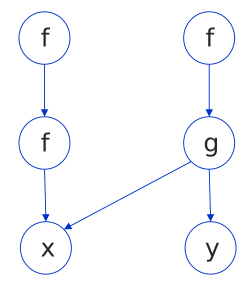
\includegraphics[scale=0.6]{figures/congruence_closure_step1.png}
	\item Füge die Prämissen hinzu
	\begin{itemize}
		\item $ x = g(x,y) $
		\item $ f(f(x)) = f(g(x,y)) $
	\end{itemize}
	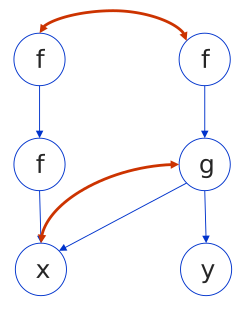
\includegraphics[scale=0.6]{figures/congruence_closure_step2.png}
	\item Wiederhole
	\begin{itemize}
		\item Bilde Kongruenzabschluss
		\begin{itemize}
			\item $ x = g(x,y)  \implies f(x) = f(g(x,y)) $
		\end{itemize}
		\item Symmetrisch-transitive Hülle
		\begin{itemize}
			\item $ x = g(x,y) \wedge f(f(x)) = f(g(x,y)) \implies f(f(x)) = f(x) $
		\end{itemize}
	\end{itemize}
	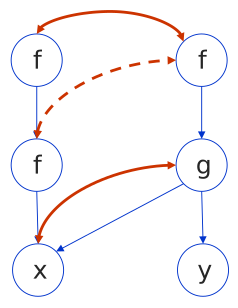
\includegraphics[scale=0.6]{figures/congruence_closure_step3.png}
	\item Lese ab, ob Konklusion besteht oder nicht \\
	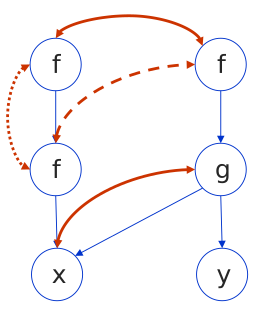
\includegraphics[scale=0.6]{figures/congruence_closure_step4.png}
\end{enumerate}

\subsection{Verbindung von Entscheidungsprozeduren}

\begin{itemize}
	\item Realistische Entscheidungsprobleme beinhalten Formeln mehrerer Theorien
	\item Beispiele \\
	\renewcommand{\arraystretch}{2}
	\begin{tabular}{l|l}
		$ f(y-1) - 1 = y + 1, f(x) + 1 = x - 1, x + 1 = y \vdash false $ & $ Th(\mathbb{Z},+,=) $, EUF \\ 
		\hline 
		$ f(f(x) - f(y)) \neq f(z), y \leq x, y \geq x + z, z \geq 0 \vdash false $ & $ Th(\mathbb{Z},+,\leq,=) $, EUF \\ 
		\hline 
		$ x + 2 = y \vdash f(a[x:=3][y-2]) = f(y-x+1) $ & $ Th(\mathbb{Z},+,=) $, EUF, Arrays \\ 
	\end{tabular}
\end{itemize}

\subsection{Nelson-Oppen}

\begin{itemize}
	\item Situation:
	\begin{itemize}
		\item Gegeben Entscheidungsverfahren $ D_1 $ für $ Th_1 $ und $ D_2 $ für $ Th_2 $
		\item Gegeben Formel $ \Phi \in L(\Sigma_1 \cup \Sigma_2) $
		\item Entkopplung in Formeln $ \Phi_1 \in L(\Sigma_1) $ und $ \Phi_2 \in L(\Sigma_2) $, so dass
		\begin{itemize}
			\item $ \Phi \vdash \bot \iff \Phi_1 \wedge \Phi_2 \vdash ? $
		\end{itemize}
		\item $ \Phi_1 $ und $ \Phi_2 $ haben zusätzliche Variablen $ x_1\ldots,x_n $
	\end{itemize}
	\item Verwende $ D_1 $ um aus $ \Phi_1 $ eine Gleichung $ x_i = x_j $ (oder eine Ungleichung $ x_i \neq x_j $) herzuleiten
	\item Verwende $ D_2 $ um aus $ \Phi_2 \cap \{ x_i = x_j \} $ eine weitere Gleichung (Ungleichung) herzuleiten
	\item Und so weiter, bis Widerspruch gefunden
\end{itemize}

\begin{equation*}
	(x_1 \leq x_2) \wedge (x_2 \leq (x_1 + car(cons(0,x_1)))) \wedge p(h(x_1) - h(x_2)) \wedge \neg p(0)
\end{equation*}

\begin{itemize}
	\item Entkopplung durch Einführung von Variablen:
	\begin{align*}
		& (x_1 \leq x_2) \wedge (x_2 \leq x_1 + a_1) \wedge p(a_2) \wedge \neg p(a_5) \wedge \\
		& a_1 = car(cons(a_5,x_1)) \wedge \\
		& a_2 = a_3 - a_4 \wedge \\
		& a_3 = h(x_1) \wedge \\
		& a_4 = h(x_2) \wedge \\
		& a_5 = 0
	\end{align*}
\end{itemize}

\begin{tabular}{|l|l|l|}
	\hline 
	Arithmetik & EUF & Listen \\ 
	\hline 
	\hline 
	$ x_1 \leq x_2 $ & $ a_3 = h(x_1) $ & $ a_1 = car(cons(a_5,x_1)) $ \\ 
	\hline 
	$ x_2 \leq x_1 + a_1 $ & $ a_4 = h(x_2) $ &  \\ 
	\hline 
	$ a_2 = a_3 - a_4 $ & $ p(a_2) $ &  \\ 
	\hline 
	$ a_5 = 0 $ & $ \neg p(a_5) $ &  \\ 
	\hline 
	\hline 
	$ a_1 = a_5 $ & $ a_1 = a_5 $ & {\cellcolor[gray]{.8}}$ a_1 = a_5 $ \\ 
	\hline 
	{\cellcolor[gray]{.8}}$ x_1 = x_2 $ & $ x_1 = x_2 $ & $ x_1 = x_2 $ \\ 
	\hline 
	$ a_3 = a_4 $ & {\cellcolor[gray]{.8}}$ a_3 = a_4 $ & $ a_3 = a_4 $ \\ 
	\hline 
	{\cellcolor[gray]{.8}}$ a_2 = a_5 $ & $ a_2 = a_5 $ & $ a_2 = a_5 $ \\ 
	\hline 
\end{tabular} \\

Da $ a_2 = a_5 $ und $ p(a_2) $, sowie $ \neg p(a_5) $ gilt $ p(0) \wedge \neg p(0) $. Dies ist trivial falsch und führt zu einem Widerspruch. Demzufolge ist die Ursprungsformel unerfüllbar.

\begin{equation*}
	\Phi := 1 \leq x \wedge x \leq 2 \wedge p(x) \wedge \neg p(1) \wedge \neg p(2), \quad x \in \mathbb{Z}
\end{equation*}

\begin{tabular}{|l|l|}
	\hline
	Arithmetik über $ \mathbb{Z} $ & Uninterpretierte Prädikate \\
	\hline 
	$ 1 \leq x $ & $ p(x) $ \\ 
	\hline 
	$ x \leq 2 $ & $ \neg p(1) $ \\ 
	\hline 
	& $ \neg p(2) $ \\ 
	\hline 
\end{tabular} 

\begin{itemize}
	\item $ x = 1 \vee x = 2 $
	\item Jede der Einzeltheorien ist erfüllbar
	\item Dennoch ist $ \Phi $ unerfüllbar!
\end{itemize}

\subsection{Konvexität}

\begin{itemize}
	\item Eine Theorie $ T $ heißt konvex, falls für jede Menge von Literalen $ L $ und je zwei Variablengleichungen $ x_1 = y_1, x_2 = y_2 $ gilt:
	\begin{itemize}
		\item Wenn $ T,L \vdash x_1 = y_1 \vee x_2 = y_2 $, dann $ T,L \vdash x_1 = y_1 $ oder $ T,L \vdash x_2 = y_2 $
	\end{itemize}
	\item Beispiel:
	\begin{itemize}
		\item $ Th(\mathbb{R},0,1,+,-,=) $ ist konvex
		\begin{itemize}
			\item Lösungen von Gleichungen sind affine Unterräume
			\item Ist ein affiner Unterraum enthalten in einer Vereinigung von zwei Unterräumen, dann auch in einem davon.
		\end{itemize}
		andererseits
		\item $ Th(\mathbb{Z},0,1,+,-,\leq,=) $ ist nicht konvex
		\begin{itemize}
			\item denn z.B. $ 1 \leq x \wedge x \leq 2 \rightarrow x = 1 \vee x = 2 $
			\begin{itemize}
				\item aber nicht $ 1 \leq x \wedge x \leq 2 \rightarrow x = 1 $
				\item und nicht $ 1 \leq x \wedge x \leq 2 \rightarrow x = 2 $
			\end{itemize}
		\end{itemize}
	\end{itemize}
\end{itemize}

\subsection{Z3}

\pagebreak
\section{Intuitionistische Logik}

\subsection{Intuitionistisches Aussagenkalkül}

\Huge
\begin{longtable}{|c|c|} 
	\hline
	$ \frac{}{\Gamma, \varphi \vdash \varphi} $ & Axiom \\
	\hline 
	$ \frac{\Gamma, \varphi \vdash \varPsi}{\Gamma, \varphi, \Delta \vdash \varPsi} $ & weakening \\ 
	\hline 
	$ \frac{\Gamma, \varphi_1, \varphi_2 \vdash \varPsi}{\Gamma, \varphi_2, \varphi_1 \vdash \varPsi} $ & Perm \\ 
	\hline 
	$ \frac{\Gamma, \varphi, \varphi \vdash \varPsi}{\Gamma, \varphi \vdash \varPsi} $ & Kontraktion \\ 
	\hline 
	$ \frac{\Gamma \vdash \varphi_1 \quad \Gamma \vdash \varphi_2}{\Gamma \vdash \varphi_1 \wedge \varphi_2} $ & $ \wedge $-intro \\
	\hline
	$ \frac{\Gamma \vdash \varphi_1 \wedge \varphi_2}{\Gamma \vdash \varphi_1} $ & $ \wedge $-elim-l \\
	\hline
	$ \frac{\Gamma \vdash \varphi_1 \wedge \varphi_2}{\Gamma \vdash \varphi_2} $ & $ \wedge $-elim-r \\
	\hline
	$ \frac{\Gamma, \varphi \vdash \varPsi}{\Gamma \vdash \varphi \rightarrow \varPsi} $ & $ \rightarrow $-intro \\
	\hline
	$ \frac{\Gamma \vdash \varphi \rightarrow \varPsi \quad \Gamma \vdash \varphi}{\Gamma \vdash \varPsi} $ & $ \rightarrow $-elim \\
	\hline
	$ \frac{\Gamma \vdash \varphi_1}{\Gamma \vdash \varphi_1 \vee \varphi_2} $ & $ \vee $-intro-l \\
	\hline
	$ \frac{\Gamma \vdash \varphi_2}{\Gamma \vdash \varphi_1 \vee \varphi_2} $ & $ \vee $-intro-l \\
	\hline
	$ \frac{\Gamma \vdash \varphi_1 \vee \varphi_2 \quad \Gamma, \varphi_1 \vdash \varPsi \quad \Gamma, \varphi_2 \vdash \varPsi}{\Gamma \vdash \varPsi} $ & $ \vee $-elim \\
	\hline
	$ \frac{\Gamma \vdash \bot}{\Gamma \vdash \varphi} $ & $ \bot $-elim \\
	\hline
	$ \frac{\Gamma, \varphi \vdash \bot}{\Gamma \vdash \neg \varphi} $ & $ \neg $-intro \\
	\hline
	$ \frac{\Gamma \vdash \neg \varphi}{\Gamma, \varphi \vdash \bot} $ & $ \neg $-elim \\
	\hline
\end{longtable}

\subsection{Tertium non datur}

\normalsize
\begin{itemize}
	\item Die bisherigen Regeln definieren den intuitionistischen Aussagenkalkül
	\item Die folgenden Regeln lassen sich damit \textbf{nicht} herleiten
	\begin{itemize}
		\item Tertium non datur (principle of excluded middle) \\
		\begin{tabular}{|c|c|}
			\hline 
			$ \frac{}{\Gamma \vdash \varphi \vee \neg \varphi} $ & PEM \\ 
			\hline 
		\end{tabular} 
		\item Reductio ad absurdum (Widerspruchsbeweis) \\
		\begin{tabular}{|c|c|}
			\hline 
			$ \frac{}{\Gamma \vdash \neg \neg \varphi \rightarrow \varphi} $ & RAA \\ 
			\hline 
		\end{tabular} 
	\end{itemize}
\end{itemize}

\subsection{Intuitionistisch (nicht) beweisbare Aussagen}

\begin{itemize}
	\item Folgende Aussagen sind intuitionistisch \textbf{nicht} beweisbar \\
	\LARGE
	\begin{tabular}{|c|c|}
		\hline 
		$ \varphi \vee \neg \varphi $ & Tertium non datur \\ 
		\hline 
		$ \neg \neg \varphi \rightarrow \varphi $ & Reductio ad absurdum \\ 
		\hline 
		$ \neg (\varphi \wedge \varPsi) \iff \neg \varphi \vee \neg \varPsi $ & deMorgan-$ \wedge $ \\ 
		\hline 
		$ \neg \varphi \vee \varPsi \iff (\varphi \rightarrow \varPsi) $ &  \\ 
		\hline 
		$ ((\varphi \rightarrow \varPsi) \rightarrow \varphi) \rightarrow \varphi $ & Peirce-Formel \\ 
		\hline 
	\end{tabular} 
	\normalsize
	\item Folgende Aussagen \textbf{sind} intuitionistisch beweisbar \\
	\LARGE
	\begin{tabular}{|c|c|}
		\hline 
		$ \varphi \rightarrow \neg \neg \varphi $ &  \\ 
		\hline 
		$ \neg \neg \neg \varphi \rightarrow \neg \varphi $ &  \\ 
		\hline 
		$ \neg(\varphi \vee \varPsi) \iff \neg \varphi \wedge \neg \varPsi $ & deMorgan-$ \vee $ \\ 
		\hline 
	\end{tabular} 
\end{itemize}

\subsection{Intuitionistische Prädikatenlogik}

\Huge
\begin{tabular}{|c|c|}
	\hline 
	$ \frac{\Gamma \vdash \varphi(x), \quad x \not \in FV(\Gamma)}{\Gamma \vdash \forall x.\varphi(x)} $ & $ \forall $-intro \\ 
	\hline 
	$ \frac{\Gamma \vdash \forall x.\varphi(x)}{\Gamma \vdash \varphi(t)} $ & $ \forall $-elim \\ 
	\hline 
	$ \frac{\Gamma \vdash \varphi(t)}{\Gamma \vdash \exists x.\varphi(x)} $ & $ \exists $-intro \\
	\hline
	$ \frac{\Gamma \vdash \exists x.\varphi(x) \quad \Gamma, \varphi(x) \vdash \varPsi \quad x \not \in FV(\Gamma)}{\Gamma \vdash \varPsi} $ & $ \exists $-elim \\
	\hline
\end{tabular} 

\subsection{Was gilt - was gilt nicht?}

\normalsize
\begin{itemize}
	\item Es gilt: $ \neg \exists x.\varphi(x) \iff \forall x. \neg \varphi(x) $
	\item Es gilt \textbf{nicht}: $ \neg \forall x.\varphi(x) \iff \exists x.\neg \varphi(x) $
\end{itemize}

\subsection{Wie zeigt man Nicht-Beweisbarkeit?}

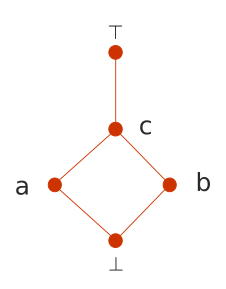
\includegraphics{figures/heyting.png}

\begin{itemize}
	\item Ersetze $ bool = \{ \bot,\top\ \} $ durch eine Heyting Algebra, z.B. $ H = \{ \bot,\top,a,b,c \} $ mit der Ordnung der Figur. Wir definieren $ \wedge,\vee,\rightarrow $ durch
	\begin{itemize}
		\item $ x \vee y = min\{ z \mid x \leq z, y \leq z \} $
		\item $ x \wedge y = max\{ z \mid z \leq x, z \leq y \} $
		\item $ x \rightarrow y = max\{ z \mid x \wedge z \leq y \} $
	\end{itemize}
	\item Insbesondere folgt:
	\begin{itemize}
		\item $ \neg c = c \rightarrow \bot = \bot $
		\item $ \neg \neg c = \bot \rightarrow \bot = \top $
	\end{itemize}
	\item Für alle $ x \neq c $ gilt $ \neg \neg x = x $
\end{itemize}

\begin{tabular}{|c|c|c|c|c|c|}
	\hline 
	$ \rightarrow $ & $ \bot $ & a & b & c & $ \top $ \\ 
	\hline 
	$ \bot $ & $ \top $ & $ \top $ & $ \top $ & $ \top $ & $ \top $ \\ 
	\hline 
	a & b & $ \top $ & b & $ \top $ & $ \top $ \\ 
	\hline 
	b & a & a & $ \top $ & $ \top $ & $ \top $ \\ 
	\hline 
	c & $ \bot $ & a & b & $ \top $ & $ \top $ \\ 
	\hline 
	$ \top $ & $ \bot $ & a & b & c & $ \top $ \\ 
	\hline 
\end{tabular} 

\end{document}